\documentclass{standalone}

\usepackage{tikz}
    \usetikzlibrary{arrows.meta}
    \usetikzlibrary{calc}
    \usetikzlibrary {decorations.pathmorphing}
    
\tikzset{
    bluearrow/.style={
        blue!25,
        -{Kite[length=2.5mm]}, 
        line width=0.5mm,},
    greensq/.style={
        green,
        fill=green!20, 
        line width=0.4mm,},
    redsq/.style={
        red,
        fill=red!20, 
        line width=0.4mm,},
    }
    
\begin{document}
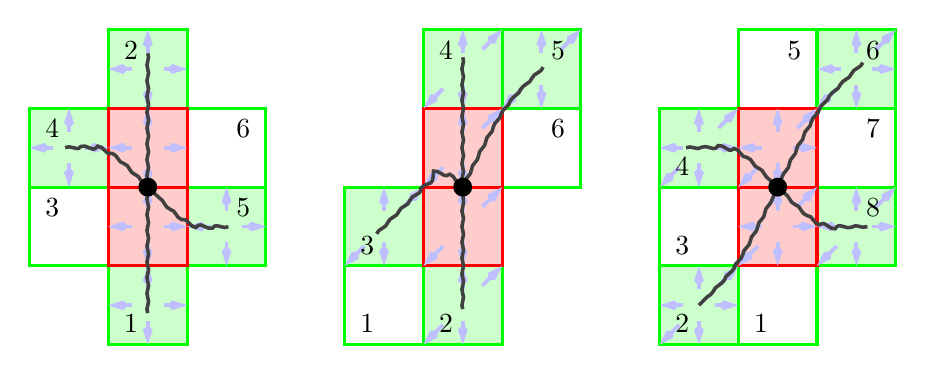
\begin{tikzpicture}
    % \draw[help lines] (0,-1) grid (15,3);
    
    \foreach \x in
        {(1,-1), (0,1),  (2,0), (1,2), % case (A) green
         (5,-1), (4,0),  (5,2), (6,2), % case (C) green
         (8,-1), (10,0), (8,1),  (10,2) % case (D6) green
        } 
        {\draw[greensq] \x rectangle+(1,1);}
    \foreach \x in
        {(0,0), (2,1), 
         (4,-1), (6,1), 
         (9,-1), (8,0), (10,1), (9,2)} 
        {\draw[green, line width=0.4mm] \x rectangle+(1,1);}
    \foreach \x in
        {(1,0), (1,1), % case (A) red
         (5,0), (5,1), % case (C) red
         (9,1), (9,0) % case (D6) red
        } 
        {\draw[redsq] \x rectangle+(1,1);}
    
    % case (A) bound
    \foreach \x in
        {(1,-1), (0,1), (2,0), (1,2), (1,0), (1,1)} 
        {\draw[bluearrow] \x++(0.3,0.5) -- ++(-0.3,0);
         \draw[bluearrow] \x++(0.7,0.5) -- ++(0.3,0);
         \draw[bluearrow] \x++(0.5,0.3) -- ++(0,-0.3);
         \draw[bluearrow] \x++(0.5,0.7) -- ++(0,0.3);}  
    % case (C) bound
    \foreach \x in
        {(5,-1), (4,0), (5,2), (6,2), (5,0), (5,1)} 
        {\draw[bluearrow] \x++(0.25,0.25) -- ++(-0.25,-0.25);
         \draw[bluearrow] \x++(0.75,0.75) -- ++(.25,0.25);
         \draw[bluearrow] \x++(0.5,0.3) -- ++(0,-0.3);
         \draw[bluearrow] \x++(0.5,0.7) -- ++(0,0.3);}
    % case (D6) bound
    \foreach \x in
        {(8,-1), (10,0), (8,1), (10,2), (9,0), (9,1)}
        {\draw[bluearrow] \x++(0.25,0.25) -- ++(-0.25,-0.25);
         \draw[bluearrow] \x++(0.75,0.75) -- ++(.25,0.25);
         \draw[bluearrow] \x++(0.3,0.5) -- ++(-0.3,0);
         \draw[bluearrow] \x++(0.7,0.5) -- ++(0.3,0);
         \draw[bluearrow] \x++(0.5,0.3) -- ++(0,-0.3);
         \draw[bluearrow] \x++(0.5,0.7) -- ++(0,0.3);}
    
    \draw[black!75, line width=0.45mm, decorate, decoration={coil, aspect=0, segment length=2mm, amplitude=0.1mm}]
        % case (A) arcs
        (1.5,1)--(1.5,-0.5) 
        (1.5,1)--(1.5,2.5) 
        %(1.5,1)..controls(1,0.5)..(0.5,0.5) 
        (1.5,1)..controls(2,0.5)..(2.5,0.5)
        (1.5,1)..controls(1,1.5)..(0.5,1.5) 
        %(1.5,1)..controls(2,1.5)..(2.5,1.5) 
        % case (C) arcs
        (5.5,1)--(5.5,2.5) 
        (5.5,1)--(5.5,-0.5)
        (5.5,1)..controls(6,2)..(6.5,2.5)  
        %(5.5,1)..controls(5.75,0.75)..(6.5,1.5) 
        %(5.5,1)..controls(5,0)..(4.5,-0.5)
        (5.5,1)..controls(5.25,1.25)..(4.5,0.5)
        % case (D6) arcs
        (9.5,1)..controls(10,2)..(10.5,2.5)
        (9.5,1)..controls(10,0.5)..(10.5,0.5)
        (9.5,1)..controls(9,1.5)..(8.5,1.5)
        (9.5,1)..controls(9,0)..(8.5,-0.5)
        ;
        
    \fill[black] 
        (1.5,1) circle (1.2mm)
        (5.5,1) circle (1.2mm)
        (9.5,1) circle (1.2mm);
        
    % A numbers
    \node[shift={(1.5,-0.5)},below left] {$1$};
    \node[shift={(1.5,2.5)},above left] {$2$};
    \node[shift={(0.5,0.5)},above left] {$3$};
    \node[shift={(0.5,1.5)},above left] {$4$};
    \node[shift={(2.5,0.5)},above right] {$5$};
    \node[shift={(2.5,1.5)},above right] {$6$};
    % C numbers
    \node[shift={(4.5,-0.5)},below left] {$1$};
    \node[shift={(5.5,-0.5)},below left] {$2$};
    \node[shift={(4.5,0.5)},below left] {$3$};
    \node[shift={(5.5,2.5)},above left] {$4$};
    \node[shift={(6.5,2.5)},above right] {$5$};
    \node[shift={(6.5,1.5)},above right] {$6$};
    % D6 numbers
    \node[shift={(9.5,-0.5)},below left] {$1$};
    \node[shift={(8.5,-0.5)},below left] {$2$};
    \node[shift={(8.5,0.5)},below left] {$3$};
    \node[shift={(8.5,1.5)},below left] {$4$};
    \node[shift={(9.5,2.5)},above right] {$5$};
    \node[shift={(10.5,2.5)},above right] {$6$};
    \node[shift={(10.5,1.5)},above right] {$7$};
    \node[shift={(10.5,0.5)},above right] {$8$};
\end{tikzpicture}
\end{document}